\documentclass[t]{beamer}

\usepackage{cite}
\usepackage{float}
\usepackage{graphicx}
\usepackage[caption=false]{subfig}
  \DeclareGraphicsExtensions{.png}
\usepackage{amsmath}
\usepackage{amsfonts}
\usepackage{url}
\usepackage[edges]{forest}
\usepackage{tikz}
\usetikzlibrary{shapes,shapes.gates.logic.US,arrows,arrows.meta,chains,calc}
\tikzset{
  -|-/.style={
    to path={
      (\tikztostart) -| ($(\tikztostart)!#1!(\tikztotarget)$) |- (\tikztotarget)
      \tikztonodes
    }
  },
  -|-/.default=0.5,
  |-|/.style={
    to path={
      (\tikztostart) |- ($(\tikztostart)!#1!(\tikztotarget)$) -| (\tikztotarget)
      \tikztonodes
    }
  },
  |-|/.default=0.5,
}
\usepackage{tikz-timing}
\usetikztiminglibrary[new={char=Q,reset char=R}]{counters}
\usepackage{bm,times}
\usepackage{pgfgantt}
\usepackage{indentfirst}
\usepackage{array}
\usepackage{setspace}
\usepackage{caption}
\usepackage{rotating}
\usepackage{hyperref}
\makeatletter
\newcommand{\verbatimfont}[1]{\renewcommand{\verbatim@font}{\ttfamily#1}}
\makeatother

%\usetheme{Boadilla}
\usetheme{Hannover}
\mode<presentation>
{
  \usetheme{default}   % or try Darmstadt, Madrid, Warsaw, ...
  \usecolortheme{default} % or try albatross, beaver, crane, ...
  \usefonttheme{default}  % or try serif, structurebold, ...
  \setbeamertemplate{navigation symbols}{}
  \setbeamertemplate{caption}[numbered]
}

\AtBeginSection[]{
  \begin{frame}
  \vfill
  \centering
  \begin{beamercolorbox}[sep=8pt,center,shadow=true,rounded=true]{title}
    \usebeamerfont{title}\insertsectionhead\par%
  \end{beamercolorbox}
  \vfill
  \end{frame}
}

\title[AAA]{An Extensible Framework for\\At-Speed Evaluation of\\Arithmetic Hardware}
\subtitle{}
\author[Zifan Wang]{Zifan Wang \texorpdfstring{\\}{} Supervisor: Dr. James Davis}
\institute[]{Imperial College London}
\date{\today}

\begin{document}

\begin{frame}
  \titlepage
\end{frame}

\begin{frame}
  \tableofcontents
\end{frame}

\section{Background}

\begin{frame}{Motivation}
  \begin{itemize}
    \item<+-> Started as a specialised evaluation system for high-radix online arithmetic units
    \begin{itemize}
      \item At-speed (Overclockable)
      \item Precision Checking
    \end{itemize}
    \item<+-> Digital designers all use their own testbenches
    \item<+-> Ad hoc, one-time use, inefficient \newline
    \item<+-> Propose an extensible framework
    \begin{itemize}
      \item With variable frequency with a high maximum (Assume DUT @300MHz)
      \item Extensible
      \item User-friendly
    \end{itemize}
  \end{itemize}
\end{frame}

\section{Design \& Implementation}

\begin{frame}{Hardware Choice}
  Cyclone V SX SoC Development Board
  \begin{figure}[H]
    \centering
    \resizebox{0.8\textwidth}{!}{%
      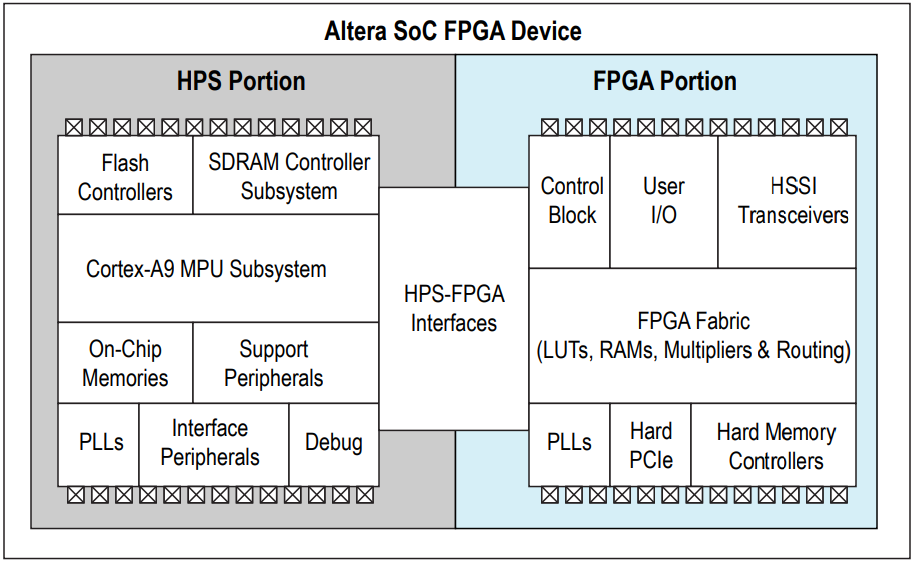
\includegraphics{img/SoCStructure}
    }
  \end{figure}
  \begin{itemize}
    \item HPS -- user interaction and test control
    \item FPGA -- actual hardware testing
  \end{itemize}
\end{frame}

\begin{frame}{System Architecture}
  \begin{itemize}
    \item Inspired by UVM agent
    \item Modular, thus extensible
  \end{itemize}
  \begin{figure}[H]
    \centering
    \resizebox{0.8\textwidth}{!}{%
      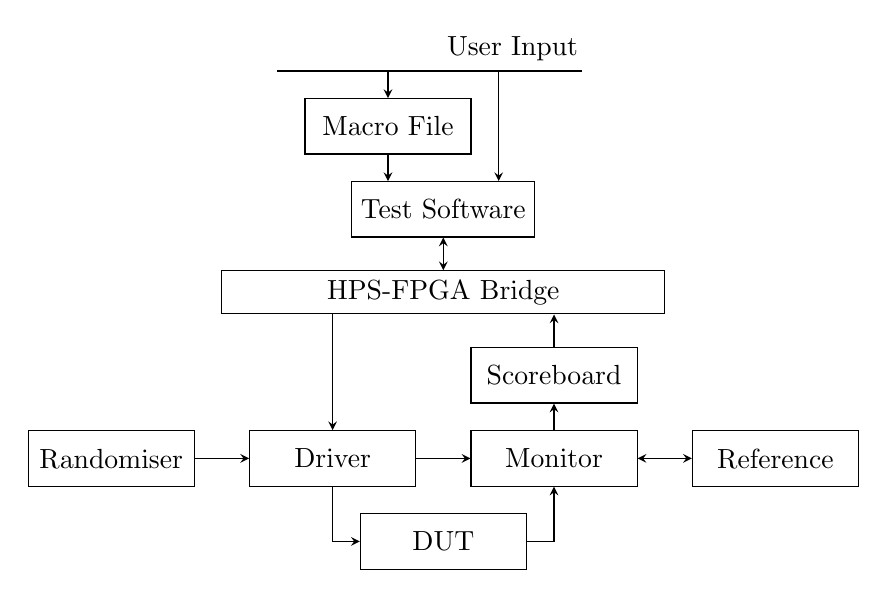
\begin{tikzpicture}
  [
    x=1em, y=1em,
    block/.style =
      {draw, rectangle, align=center, minimum width=6em, minimum height=2em},
    inter/.style =
      {draw, rectangle, align=center, minimum width=16em, minimum height=1em}
  ]
  \node [block] at (-8,3)  (r) {Randomiser};
  \node [block] at ( 0,3)  (d) {Driver};
  \node [block] at ( 4,0)  (t) {DUT};
  \node [block] at ( 8,6)  (s) {Scoreboard};
  \node [block] at ( 8,3)  (m) {Monitor};
  \node [block] at (16,3)  (u) {Reference};
  \node [inter] at ( 4,9)  (b) {HPS-FPGA Bridge};
  \node [block] at ( 4,12) (w) {Test Software};
  \node [block] at ( 2,15) (f) {Macro File};

  \draw[ ->, >=stealth] (r.east)           -- (d.west);
  \draw[ ->, >=stealth] (d.south)          |- (t.west);
  \draw[ ->, >=stealth] (t.east)           -| (m.south);
  \draw[ ->, >=stealth] (m.north)          -- (s.south);
  \draw[ ->, >=stealth] (b.south-|d.north) -- (d.north);
  \draw[ ->, >=stealth] (s.north)          -- (b.south-|s.north);
  \draw[<->, >=stealth] (b.north)          -- (w.south);
  \draw[ ->, >=stealth] (f.south)          -- (w.north-|f.north);
  \draw[ ->, >=stealth] (d.east)           -- (m.west);
  \draw[<->, >=stealth] (m.east)           -- (u.west);
  \draw[ ->, >=stealth] (2, 17)            -- (f.north);
  \draw[ ->, >=stealth] (6, 17)            -- (w.north-|6,17);

  \draw (-2,17) -- ++(6,0) -- node[above] {User Input} ++(5,0);
\end{tikzpicture}
    }
  \end{figure}
\end{frame}

\begin{frame}{System Architecture}
  \begin{figure}[H]
    \centering
    \resizebox{0.8\textwidth}{!}{%
      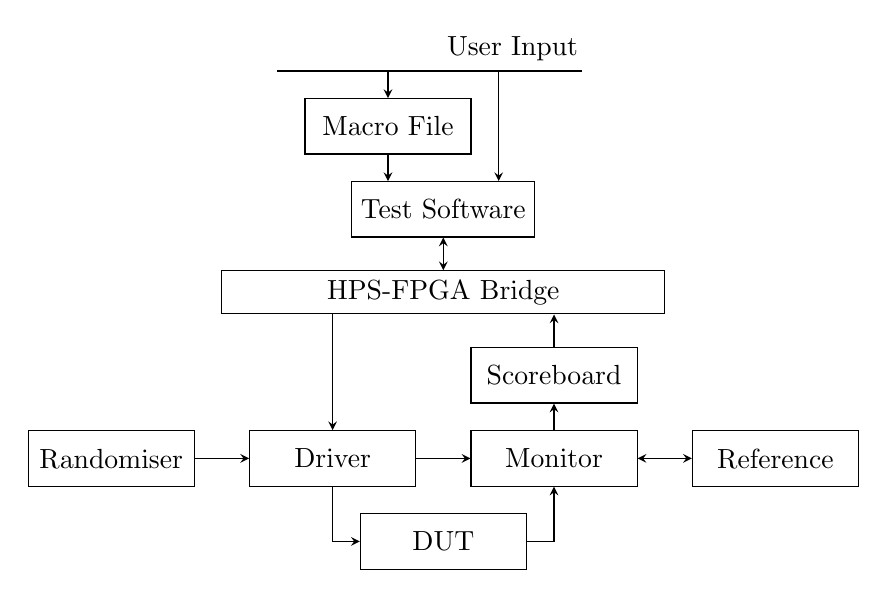
\begin{tikzpicture}
  [
    x=1em, y=1em,
    block/.style =
      {draw, rectangle, align=center, minimum width=6em, minimum height=2em},
    inter/.style =
      {draw, rectangle, align=center, minimum width=16em, minimum height=1em}
  ]
  \node [block] at (-8,3)  (r) {Randomiser};
  \node [block] at ( 0,3)  (d) {Driver};
  \node [block] at ( 4,0)  (t) {DUT};
  \node [block] at ( 8,6)  (s) {Scoreboard};
  \node [block] at ( 8,3)  (m) {Monitor};
  \node [block] at (16,3)  (u) {Reference};
  \node [inter] at ( 4,9)  (b) {HPS-FPGA Bridge};
  \node [block] at ( 4,12) (w) {Test Software};
  \node [block] at ( 2,15) (f) {Macro File};

  \draw[ ->, >=stealth] (r.east)           -- (d.west);
  \draw[ ->, >=stealth] (d.south)          |- (t.west);
  \draw[ ->, >=stealth] (t.east)           -| (m.south);
  \draw[ ->, >=stealth] (m.north)          -- (s.south);
  \draw[ ->, >=stealth] (b.south-|d.north) -- (d.north);
  \draw[ ->, >=stealth] (s.north)          -- (b.south-|s.north);
  \draw[<->, >=stealth] (b.north)          -- (w.south);
  \draw[ ->, >=stealth] (f.south)          -- (w.north-|f.north);
  \draw[ ->, >=stealth] (d.east)           -- (m.west);
  \draw[<->, >=stealth] (m.east)           -- (u.west);
  \draw[ ->, >=stealth] (2, 17)            -- (f.north);
  \draw[ ->, >=stealth] (6, 17)            -- (w.north-|6,17);

  \draw (-2,17) -- ++(6,0) -- node[above] {User Input} ++(5,0);
\end{tikzpicture}
    }
  \end{figure}
  \begin{itemize}
    \item Software accepts user commands from files or command line
  \end{itemize}
\end{frame}

\begin{frame}{System Architecture}
  \begin{figure}[H]
    \centering
    \resizebox{0.8\textwidth}{!}{%
      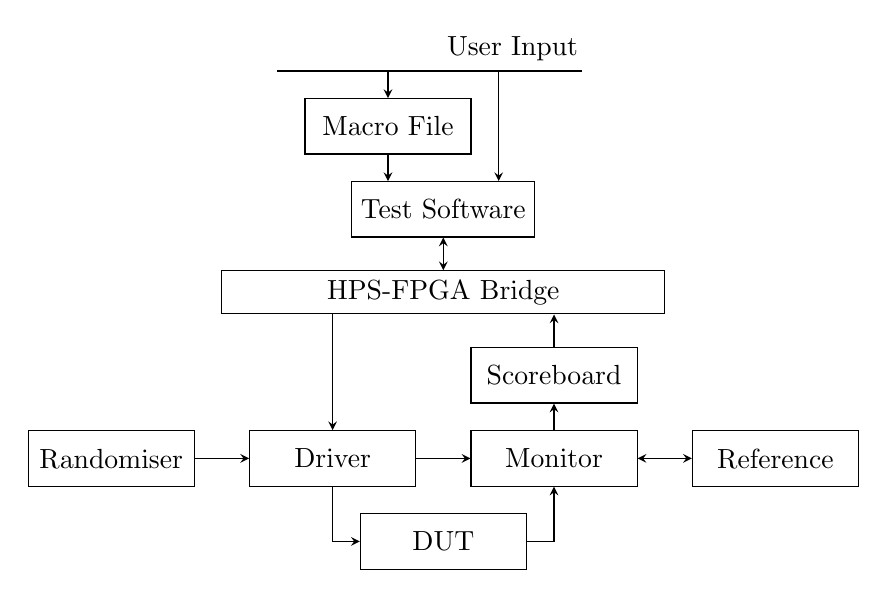
\begin{tikzpicture}
  [
    x=1em, y=1em,
    block/.style =
      {draw, rectangle, align=center, minimum width=6em, minimum height=2em},
    inter/.style =
      {draw, rectangle, align=center, minimum width=16em, minimum height=1em}
  ]
  \node [block] at (-8,3)  (r) {Randomiser};
  \node [block] at ( 0,3)  (d) {Driver};
  \node [block] at ( 4,0)  (t) {DUT};
  \node [block] at ( 8,6)  (s) {Scoreboard};
  \node [block] at ( 8,3)  (m) {Monitor};
  \node [block] at (16,3)  (u) {Reference};
  \node [inter] at ( 4,9)  (b) {HPS-FPGA Bridge};
  \node [block] at ( 4,12) (w) {Test Software};
  \node [block] at ( 2,15) (f) {Macro File};

  \draw[ ->, >=stealth] (r.east)           -- (d.west);
  \draw[ ->, >=stealth] (d.south)          |- (t.west);
  \draw[ ->, >=stealth] (t.east)           -| (m.south);
  \draw[ ->, >=stealth] (m.north)          -- (s.south);
  \draw[ ->, >=stealth] (b.south-|d.north) -- (d.north);
  \draw[ ->, >=stealth] (s.north)          -- (b.south-|s.north);
  \draw[<->, >=stealth] (b.north)          -- (w.south);
  \draw[ ->, >=stealth] (f.south)          -- (w.north-|f.north);
  \draw[ ->, >=stealth] (d.east)           -- (m.west);
  \draw[<->, >=stealth] (m.east)           -- (u.west);
  \draw[ ->, >=stealth] (2, 17)            -- (f.north);
  \draw[ ->, >=stealth] (6, 17)            -- (w.north-|6,17);

  \draw (-2,17) -- ++(6,0) -- node[above] {User Input} ++(5,0);
\end{tikzpicture}
    }
  \end{figure}
  \begin{itemize}
    \item Randomiser generate random data with LFSRs
  \end{itemize}
\end{frame}

\begin{frame}{System Architecture}
  \begin{figure}[H]
    \centering
    \resizebox{0.8\textwidth}{!}{%
      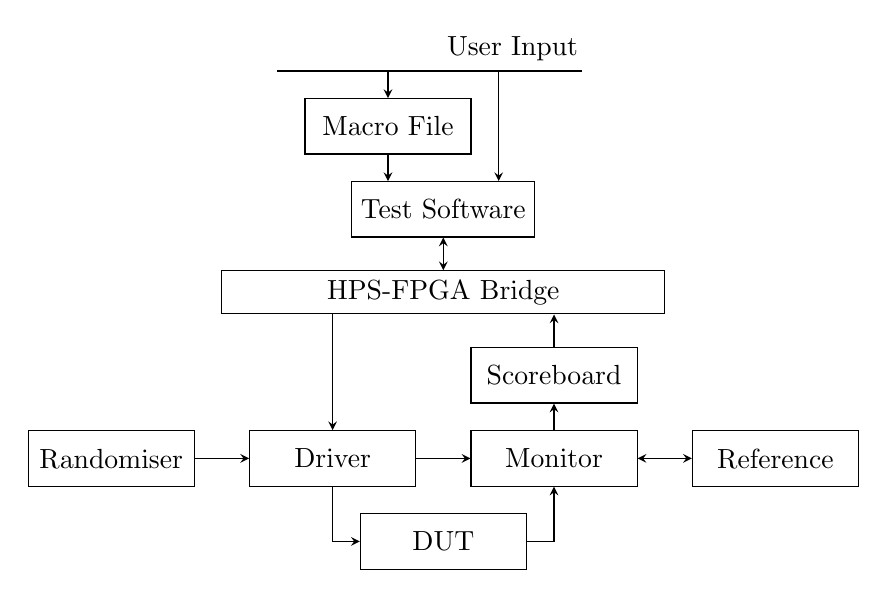
\begin{tikzpicture}
  [
    x=1em, y=1em,
    block/.style =
      {draw, rectangle, align=center, minimum width=6em, minimum height=2em},
    inter/.style =
      {draw, rectangle, align=center, minimum width=16em, minimum height=1em}
  ]
  \node [block] at (-8,3)  (r) {Randomiser};
  \node [block] at ( 0,3)  (d) {Driver};
  \node [block] at ( 4,0)  (t) {DUT};
  \node [block] at ( 8,6)  (s) {Scoreboard};
  \node [block] at ( 8,3)  (m) {Monitor};
  \node [block] at (16,3)  (u) {Reference};
  \node [inter] at ( 4,9)  (b) {HPS-FPGA Bridge};
  \node [block] at ( 4,12) (w) {Test Software};
  \node [block] at ( 2,15) (f) {Macro File};

  \draw[ ->, >=stealth] (r.east)           -- (d.west);
  \draw[ ->, >=stealth] (d.south)          |- (t.west);
  \draw[ ->, >=stealth] (t.east)           -| (m.south);
  \draw[ ->, >=stealth] (m.north)          -- (s.south);
  \draw[ ->, >=stealth] (b.south-|d.north) -- (d.north);
  \draw[ ->, >=stealth] (s.north)          -- (b.south-|s.north);
  \draw[<->, >=stealth] (b.north)          -- (w.south);
  \draw[ ->, >=stealth] (f.south)          -- (w.north-|f.north);
  \draw[ ->, >=stealth] (d.east)           -- (m.west);
  \draw[<->, >=stealth] (m.east)           -- (u.west);
  \draw[ ->, >=stealth] (2, 17)            -- (f.north);
  \draw[ ->, >=stealth] (6, 17)            -- (w.north-|6,17);

  \draw (-2,17) -- ++(6,0) -- node[above] {User Input} ++(5,0);
\end{tikzpicture}
    }
  \end{figure}
  \begin{itemize}
    \item Driver filters inputs and drives them to the DUT and the monitor
  \end{itemize}
\end{frame}

\begin{frame}{System Architecture}
  \begin{figure}[H]
    \centering
    \resizebox{0.8\textwidth}{!}{%
      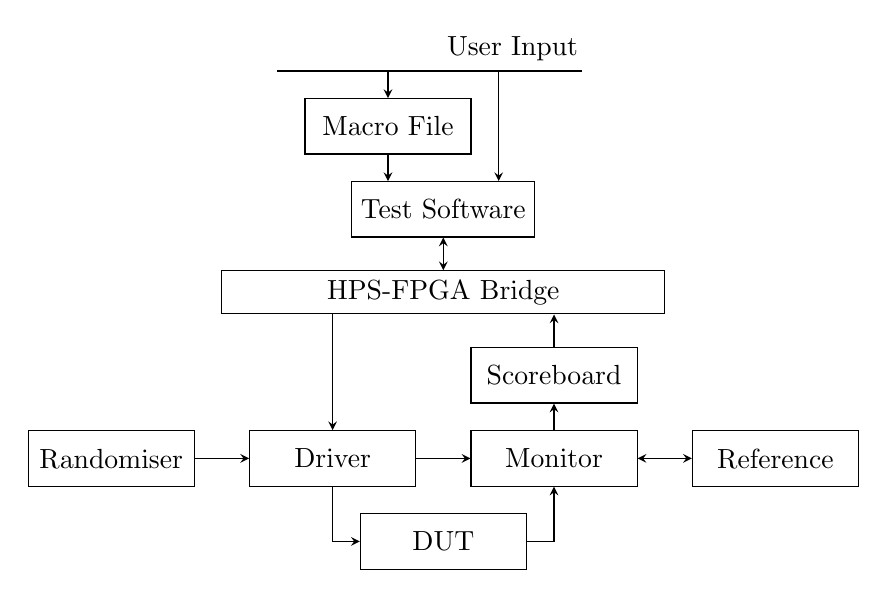
\begin{tikzpicture}
  [
    x=1em, y=1em,
    block/.style =
      {draw, rectangle, align=center, minimum width=6em, minimum height=2em},
    inter/.style =
      {draw, rectangle, align=center, minimum width=16em, minimum height=1em}
  ]
  \node [block] at (-8,3)  (r) {Randomiser};
  \node [block] at ( 0,3)  (d) {Driver};
  \node [block] at ( 4,0)  (t) {DUT};
  \node [block] at ( 8,6)  (s) {Scoreboard};
  \node [block] at ( 8,3)  (m) {Monitor};
  \node [block] at (16,3)  (u) {Reference};
  \node [inter] at ( 4,9)  (b) {HPS-FPGA Bridge};
  \node [block] at ( 4,12) (w) {Test Software};
  \node [block] at ( 2,15) (f) {Macro File};

  \draw[ ->, >=stealth] (r.east)           -- (d.west);
  \draw[ ->, >=stealth] (d.south)          |- (t.west);
  \draw[ ->, >=stealth] (t.east)           -| (m.south);
  \draw[ ->, >=stealth] (m.north)          -- (s.south);
  \draw[ ->, >=stealth] (b.south-|d.north) -- (d.north);
  \draw[ ->, >=stealth] (s.north)          -- (b.south-|s.north);
  \draw[<->, >=stealth] (b.north)          -- (w.south);
  \draw[ ->, >=stealth] (f.south)          -- (w.north-|f.north);
  \draw[ ->, >=stealth] (d.east)           -- (m.west);
  \draw[<->, >=stealth] (m.east)           -- (u.west);
  \draw[ ->, >=stealth] (2, 17)            -- (f.north);
  \draw[ ->, >=stealth] (6, 17)            -- (w.north-|6,17);

  \draw (-2,17) -- ++(6,0) -- node[above] {User Input} ++(5,0);
\end{tikzpicture}
    }
  \end{figure}
  \begin{itemize}
    \item Monitor watches for the differences between DUT and reference outputs
  \end{itemize}
\end{frame}

\begin{frame}{System Architecture}
  \begin{figure}[H]
    \centering
    \resizebox{0.8\textwidth}{!}{%
      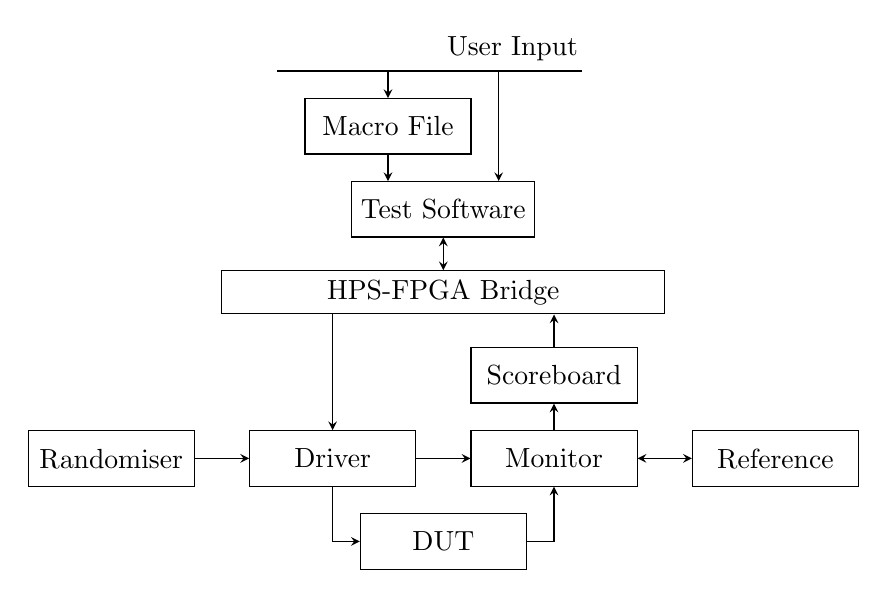
\begin{tikzpicture}
  [
    x=1em, y=1em,
    block/.style =
      {draw, rectangle, align=center, minimum width=6em, minimum height=2em},
    inter/.style =
      {draw, rectangle, align=center, minimum width=16em, minimum height=1em}
  ]
  \node [block] at (-8,3)  (r) {Randomiser};
  \node [block] at ( 0,3)  (d) {Driver};
  \node [block] at ( 4,0)  (t) {DUT};
  \node [block] at ( 8,6)  (s) {Scoreboard};
  \node [block] at ( 8,3)  (m) {Monitor};
  \node [block] at (16,3)  (u) {Reference};
  \node [inter] at ( 4,9)  (b) {HPS-FPGA Bridge};
  \node [block] at ( 4,12) (w) {Test Software};
  \node [block] at ( 2,15) (f) {Macro File};

  \draw[ ->, >=stealth] (r.east)           -- (d.west);
  \draw[ ->, >=stealth] (d.south)          |- (t.west);
  \draw[ ->, >=stealth] (t.east)           -| (m.south);
  \draw[ ->, >=stealth] (m.north)          -- (s.south);
  \draw[ ->, >=stealth] (b.south-|d.north) -- (d.north);
  \draw[ ->, >=stealth] (s.north)          -- (b.south-|s.north);
  \draw[<->, >=stealth] (b.north)          -- (w.south);
  \draw[ ->, >=stealth] (f.south)          -- (w.north-|f.north);
  \draw[ ->, >=stealth] (d.east)           -- (m.west);
  \draw[<->, >=stealth] (m.east)           -- (u.west);
  \draw[ ->, >=stealth] (2, 17)            -- (f.north);
  \draw[ ->, >=stealth] (6, 17)            -- (w.north-|6,17);

  \draw (-2,17) -- ++(6,0) -- node[above] {User Input} ++(5,0);
\end{tikzpicture}
    }
  \end{figure}
  \begin{itemize}
    \item Scoreboard tallies them and provides results to software
  \end{itemize}
\end{frame}

\begin{frame}{System Architecture}
  \begin{figure}[H]
    \centering
    \resizebox{0.8\textwidth}{!}{%
      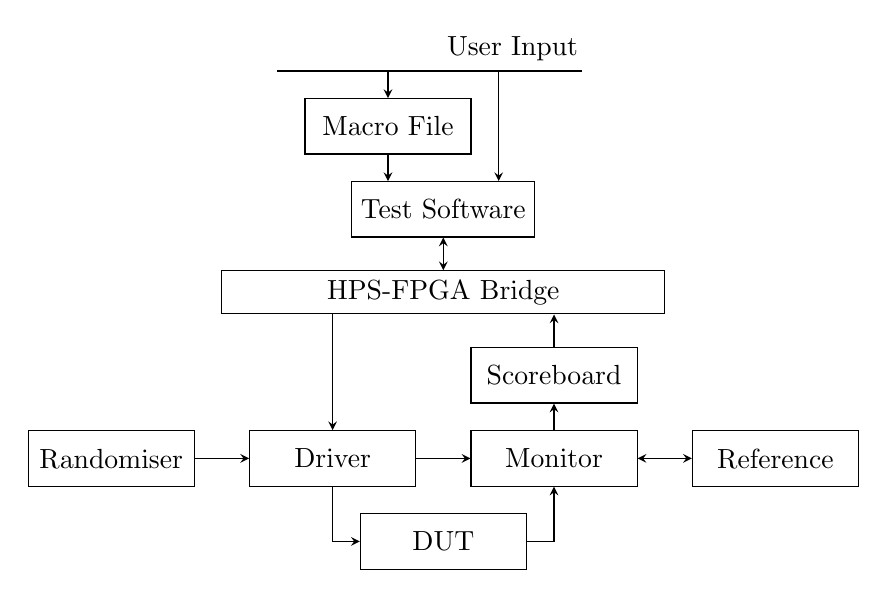
\begin{tikzpicture}
  [
    x=1em, y=1em,
    block/.style =
      {draw, rectangle, align=center, minimum width=6em, minimum height=2em},
    inter/.style =
      {draw, rectangle, align=center, minimum width=16em, minimum height=1em}
  ]
  \node [block] at (-8,3)  (r) {Randomiser};
  \node [block] at ( 0,3)  (d) {Driver};
  \node [block] at ( 4,0)  (t) {DUT};
  \node [block] at ( 8,6)  (s) {Scoreboard};
  \node [block] at ( 8,3)  (m) {Monitor};
  \node [block] at (16,3)  (u) {Reference};
  \node [inter] at ( 4,9)  (b) {HPS-FPGA Bridge};
  \node [block] at ( 4,12) (w) {Test Software};
  \node [block] at ( 2,15) (f) {Macro File};

  \draw[ ->, >=stealth] (r.east)           -- (d.west);
  \draw[ ->, >=stealth] (d.south)          |- (t.west);
  \draw[ ->, >=stealth] (t.east)           -| (m.south);
  \draw[ ->, >=stealth] (m.north)          -- (s.south);
  \draw[ ->, >=stealth] (b.south-|d.north) -- (d.north);
  \draw[ ->, >=stealth] (s.north)          -- (b.south-|s.north);
  \draw[<->, >=stealth] (b.north)          -- (w.south);
  \draw[ ->, >=stealth] (f.south)          -- (w.north-|f.north);
  \draw[ ->, >=stealth] (d.east)           -- (m.west);
  \draw[<->, >=stealth] (m.east)           -- (u.west);
  \draw[ ->, >=stealth] (2, 17)            -- (f.north);
  \draw[ ->, >=stealth] (6, 17)            -- (w.north-|6,17);

  \draw (-2,17) -- ++(6,0) -- node[above] {User Input} ++(5,0);
\end{tikzpicture}
    }
  \end{figure}
  \begin{itemize}
    \item Software reads results and present them to user
  \end{itemize}
\end{frame}

\begin{frame}{Hardware Project Hierarchy}
  \begin{itemize}[<+->]
    \item Adapted from a golden system reference design
  \end{itemize}
  \begin{figure}[H]
    \centering
    \resizebox{0.8\textwidth}{!}{%
      \begin{forest}
  for tree={
    align=center,
    font=\ttfamily,
    edge+={thick},
    l sep'+=10pt,
    fork sep'=10pt,
  },
  forked edges,
  if level=0{
    inner xsep=0pt,
    tikz={\draw [thick] (.children first) -- (.children last);}
  }{},
  [\textbf{sys\_top}
    [reset]
    [debounce]
    [\textbf{soc\_system}
      [\textbf{hps}]
      [hps\_only\_master]
      [jtag\_uart]
      [button\_pio]
      [...]
    ]
    [edge\_detector]
    [...]
  ]
\end{forest}
    }
  \end{figure}
  \begin{itemize}[<+->]
    \item Already uses \textit{Qsys} for \texttt{soc\_system}
    \item Frequency control uses \texttt{pll} (Phase-locked loop) and \texttt{pll\_reconfig} IP, easy integration with \textit{Qsys}.
    \item Great interface for user to connect their design and reference modules
  \end{itemize}

\end{frame}

\begin{frame}{Hardware Project Hierarchy}
  \begin{figure}[H]
    \centering
    \resizebox{0.8\textwidth}{!}{%
      \begin{forest}
  for tree={
    align=center,
    font=\ttfamily,
    edge+={thick},
    l sep'+=10pt,
    fork sep'=10pt,
  },
  forked edges,
  if level=0{
    inner xsep=0pt,
    tikz={\draw [thick] (.children first) -- (.children last);}
  }{},
  [sys\_top
    [reset]
    [debounce]
    [soc\_system
      [hps]
      [\textbf{pll}]
      [\textbf{pll\_reconfig}]
      [\textbf{test\_wrapper}
        [\textbf{testbench}
          [\textbf{randomiser}]
          [\textbf{driver}]
          [\textbf{monitor}
            [\textbf{sub\_mon}]
          ]
          [\textbf{scoreboard}]
        ]
      ]
      [\textbf{dut}]
      [\textbf{ref}]
      [...]
    ]
    [edge\_detector]
    [...]
  ]
\end{forest}
    }
  \end{figure}
  \begin{itemize}[<+->]
    \item Access to software through \texttt{hps}
    \item Access to hardware design through \texttt{dut} and \texttt{ref}
  \end{itemize}
\end{frame}


\begin{frame}{Providing test data}
  \begin{itemize}
    \item<+-> Assume DUT is 32-bit @300MHz, need sustained data input for stress testing \newline
    \item<+-> Real time, on board generation of random test data
    \begin{itemize}
      \item Low effort, significant coverage, can discover subtle errors
      \item Include filters to give user control
      \item Accept manual inputs from users for critical path
    \end{itemize}
  \end{itemize}
\end{frame}

\begin{frame}{Relaxed Reference}
  \begin{itemize}
    \item Monitors needs reference module to check correctness
    \item Has to be functionally correct
    \item Sensible to have reduced timing requirements
    \item Harder for users to make mistakes
  \end{itemize}
\end{frame}

\begin{frame}{Monitor Structure}
  \begin{itemize}
    \item Parallel Monitor
    \begin{itemize}
      \item Checks all data points in parallel
    \end{itemize}
  \end{itemize}
  \begin{figure}[H]
    \centering
    \resizebox{0.8\textwidth}{!}{%
      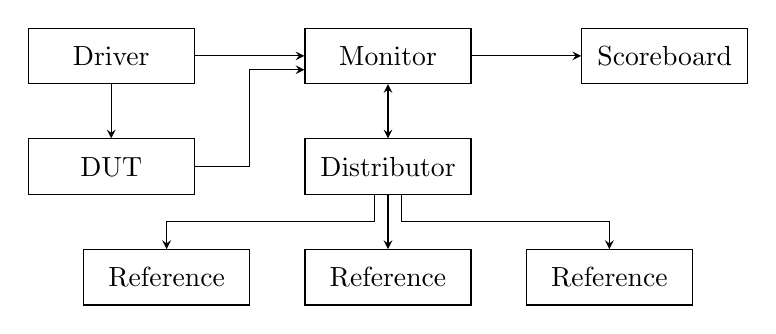
\begin{tikzpicture}
  [
    x=1em, y=1em,
    block/.style =
      {draw, rectangle, align=center, minimum width=6em, minimum height=2em},
    inter/.style =
      {draw, rectangle, align=center, minimum width=16em, minimum height=1em}
  ]
  \node [block] at ( 0,4)  (d) {Driver};
  \node [block] at ( 0,0)  (t) {DUT};
  \node [block] at (10,4)  (m) {Monitor};
  \node [block] at (10,0)  (u) {Distributor};
  \node [block] at (20,4)  (s) {Scoreboard};
  \node [block] at ( 2,-4)  (r1) {Reference};
  \node [block] at (10,-4)  (r2) {Reference};
  \node [block] at (18,-4)  (r3) {Reference};

  \draw[ ->, >=stealth] (d.east)                 -- (m.west);
  \draw[ ->, >=stealth] (d.south)                -- (t.north);
  \draw[ ->, >=stealth] (t.east)            to[-|-] ($(m.west)-(0,0.5)$);
  \draw[<->, >=stealth] (m.south)                -- (u.north);
  \draw[ ->, >=stealth] (m.east)                 -- (s.west);
  \draw[ ->, >=stealth] ($(u.south)-(0.5,0)$) to[|-|] (r1.north);
  \draw[ ->, >=stealth] ($(u.south)+(0,0)$)   to[|-|] (r2.north);
  \draw[ ->, >=stealth] ($(u.south)+(0.5,0)$) to[|-|] (r3.north);

\end{tikzpicture}
    }
  \end{figure}
\end{frame}


\begin{frame}{Software Design}
  \begin{itemize}
    \item<+-> Requirement
    \begin{itemize}
      \item Manual and auto input controls
      \item Test duration
      \item PLL frequency \newline
    \end{itemize}
    \item<+-> Considered solutions
    \begin{itemize}
      \item Test configuration files
      \begin{itemize}
        \item Easy to build and scale
        \item Slightly harder to use and manage
      \end{itemize}
      \item Interactive REPL system
      \begin{itemize}
        \item Intuitive to control
        \item Easy to automate and scale
      \end{itemize}
    \end{itemize}
  \end{itemize}
\end{frame}

\section{Results}
\begin{frame}{Results}
\begin{itemize}
  \item<+-> Maximum frequency
  \begin{itemize}
    \item TimeQuest: 394.01MHz
    \item Hardware test: Stable at 400MHz; breaks at 425MHz
    \item DUT initially assume to work at 300MHz \newline
  \end{itemize}
  \item<+-> User-friendliness
  \begin{itemize}
    \item Performed an OOTB Testing
    \item Knowledge of digital designs and testbenches
    \item No previous knowledge on Qsys or the framework
    \item Obtained results in 2 hours
    \item No major interruptions, positive feedback \newline
  \end{itemize}
  \item<+-> Flexibility
\end{itemize}
\end{frame}

\begin{frame}{Flexibility}
  \begin{table}[H]
    \centering
    \begin{tabular}{|l|c|}
      \hline
      Item                  & Reconfigurability \\
      \hline
      \texttt{WIDTH}        & $\le$32 bits \\
      \texttt{NUM\_SUB\_MON}& $\ge$2       \\
      $f_{\text{dut}}$      & $\le$400MHz  \\
      DUT I/O               & 2 in 1 out   \\
      DUT delay             & All values   \\
      bitset/bitclr         & All values   \\
      manual                & All values   \\
      time                  & All values   \\
      \hline
    \end{tabular}
  \end{table}
\end{frame}

\begin{frame}{Demo}
  \begin{itemize}
    \item Shows the configuration process
    \item Shows software interaction
  \end{itemize}
  \begin{table}[H]
    \centering
    \begin{tabular}{|>{\ttfamily\scriptsize}p{8em}|>{\scriptsize}p{\dimexpr\textwidth-12em}|}
      \hline
      \textrm{Command}   & Explanation \\
      \hline
      reset              & Resets the system and test results. \\
      version            & Prints the system version. \\
      freq <speed>       & Sets the clock speed to the specified value in MHz. Prints the actual frequency configured. \\
      mode <m|a>         & Choose between \underline{m}anual and \underline{a}uto test mode. \\
      manual <a|b> <hex> & Give input in manual mode. \\
      bitset <a|b> <hex> & Force bits to be 1 in auto mode. \\
      bitclr <a|b> <hex> & Force bits to be 0 in auto mode. \\
      run <time>         & Runs the test for the duration specified in seconds. Prints the results at the end of the test. \\
      exit               & Exits the REPL. \\
      \hline
    \end{tabular}
  \end{table}
\end{frame}

\section{Evaluation}

\begin{frame}{What have we done?}
  \begin{figure}[H]
    \centering
    \resizebox{\textwidth}{!}{%
      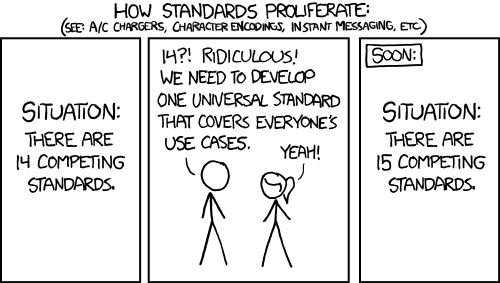
\includegraphics{img/standards}
    }
  \end{figure}
  \small{xkcd.com/927}
\end{frame}

\begin{frame}{Evaluation}
\begin{itemize}
  \item<+-> Limitations
  \begin{itemize}
    \item Customisability of current implementation
  \end{itemize}
  \item<+-> Improvements
  \begin{itemize}
    \item User experience can be made better with a unified software system + Verilog preprocessor
    \item Set up a more powerful HPS-FPGA communication system to allow more insightful results \newline
  \end{itemize}
  \item<+-> Not limits to the extensibility of the framework
\end{itemize}
\end{frame}

\begin{frame}{Thank you}
  Questions?
\end{frame}

\section{Backup Slides}

\begin{frame}{Providing test data}
  \begin{itemize}
    \item Assume 32-bit @600MHz, need sustained 19.2Gbps for stress testing
    \item HPS-FPGA bridge
    \begin{itemize}
      \item Assume perfect packing and always burst transfer
      \item 128-bit @133MHz, 17.0Gbps
    \end{itemize}
    \item Off-chip SDRAM
    \begin{itemize}
      \item Assume always burst, access pipelined
      \item 32-bit DDR3 @400MHz, 25.6Gbps
      \item Sufficient, but needs time to fill up
      \item SDRAM controller can be complex to use and manage
    \end{itemize}
    \item On-chip memory
    \begin{itemize}
      \item Assume widest possible arrangement
      \item 768.9kB @315MHz, 242Gbps
      \item Very fast, but extremely small capacity for sustained load
    \end{itemize}
    \item Real time generation
  \end{itemize}
\end{frame}

\begin{frame}{LFSRs}
  \begin{figure}[H]
    \centering
    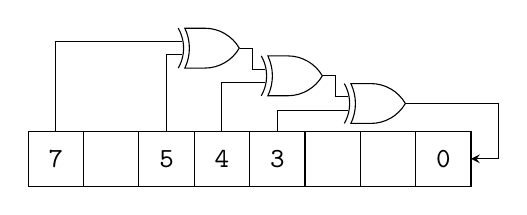
\begin{tikzpicture}
  [
    x=1em, y=1em,
    start chain = going left,
    node distance = 0em,
    reg/.style =
      {draw, minimum width=2em, minimum height=2em,outer sep=0pt, on chain},
    every join/.style={-, thick}
  ]
  \node [reg] at (0, 0) (1) {\texttt{0}};
  \node [reg] (2) {};
  \node [reg] (3) {};
  \node [reg] (4) {\texttt{3}};
  \node [reg] (5) {\texttt{4}};
  \node [reg] (6) {\texttt{5}};
  \node [reg] (7) {};
  \node [reg] (8) {\texttt{7}};

  \node [xor gate US,draw] at (-2.5, 2) (a) {};
  \node [xor gate US,draw] at (-5.5, 3) (b) {};
  \node [xor gate US,draw] at (-8.5, 4) (c) {};

  \draw (b.output) to[-|-] (a.input 1);
  \draw (c.output) to[-|-] (b.input 1);
  \draw (8.north)       |- (c.input 1);

  \draw (4.north)  |- (a.input 2);
  \draw (5.north)  |- (b.input 2);
  \draw (6.north)  |- (c.input 2);

  \draw [->, >=stealth] (a.output) -- (2, 2) |- (1.east);

\end{tikzpicture}
  \end{figure}
  \begin{figure}[H]
    \centering
    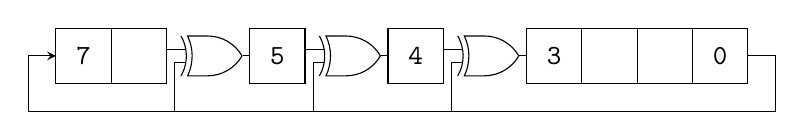
\begin{tikzpicture}
  [
    x=1em, y=1em,
    start chain = going left,
    node distance = 0em,
    reg/.style =
      {draw, minimum width=2em, minimum height=2em, outer sep=0pt, on chain},
    spa/.style =
      {minimum width=3em, minimum height=2em, outer sep=0pt, on chain},
    every join/.style={-, thick}
  ]
  \node [reg] at (0, 0) (1) {\texttt{0}};
  \node [reg] (2) {};
  \node [reg] (3) {};
  \node [reg] (4) {\texttt{3}};
  \node [spa] ()  {};
  \node [reg] (5) {\texttt{4}};
  \node [spa] ()  {};
  \node [reg] (6) {\texttt{5}};
  \node [spa] ()  {};
  \node [reg] (7) {};
  \node [reg] (8) {\texttt{7}};

  \node [xor gate US,draw] at  (-8.4, 0) (a) {};
  \node [xor gate US,draw] at (-13.4, 0) (b) {};
  \node [xor gate US,draw] at (-18.4, 0) (c) {};

  \draw [->, >=stealth] (1.east) -| (2, -2) -- (-25,-2) |- (8.west);

  \draw (a.input 1-|5.east) -- (a.input 1);
  \draw (b.input 1-|6.east) -- (b.input 1);
  \draw (c.input 1-|7.east) -- (c.input 1);

  \draw  (-9.7,-2) |- (a.input 2);
  \draw (-14.7,-2) |- (b.input 2);
  \draw (-19.7,-2) |- (c.input 2);

  \draw (a.output) -- (4.west);
  \draw (b.output) -- (5.west);
  \draw (c.output) -- (6.west);

\end{tikzpicture}
  \end{figure}
\end{frame}

\begin{frame}{Randomiser Structure}
  \begin{figure}[H]
    \centering
    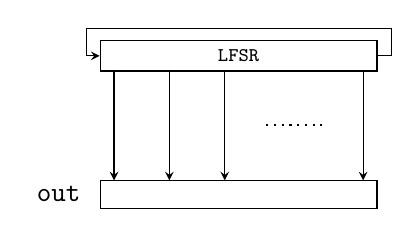
\begin{tikzpicture}
  [
    x=1em, y=1em
  ]
  \node at (-1.5, 0) {\texttt{out}};
  \node [draw,minimum height=1em, minimum width=10em] at (5, 0) (o) {};
  \node [draw,minimum height=1em, minimum width=10em] at (5, 5) (1) {\scriptsize \texttt{LFSR}};
  \draw [->, >=stealth] (1.east) -| ++(0.5, 1) -- ++(-11, 0) |- (1.west);
  \foreach \pos [count=\idx] in {0.5, 2.5, 4.5, 9.5}{
    \draw [->, >=stealth] (\pos, 4.5) -- (\pos, 0.5);
  }
  \draw [dotted, thick] (6, 2.5) -- (8, 2.5);

\end{tikzpicture}
  \end{figure}
  \begin{figure}[H]
    \centering
    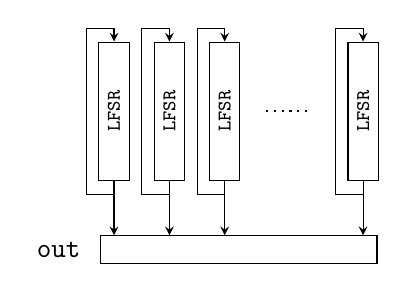
\begin{tikzpicture}
  [
    x=1em, y=1em
  ]
  \node at (-1.5, 0) {\texttt{out}};
  \node [draw,minimum height=1em, minimum width=10em] at (5, 0) (o) {};
  \foreach \pos [count=\idx] in {0.5, 2.5, 4.5, 9.5}{
    \node [draw,minimum height=1em, minimum width=5em, rotate around={90:(0, 0)}] at (\pos, 5) (\idx) {\scriptsize \texttt{LFSR}};
    \draw [->, >=stealth] (\idx.west) -- (\idx.west|-o.north);
    \draw [->, >=stealth] ($(\idx.west)-(0, 0.5)$) -| (\pos-1,8) -| (\idx.east);
  }

  \draw [dotted, thick] (6, 5) -- (7.5, 5);

\end{tikzpicture}
  \end{figure}
\end{frame}

\begin{frame}{Hardware}
  \begin{figure}[H]
    \centering
    \resizebox{\textwidth}{!}{%
      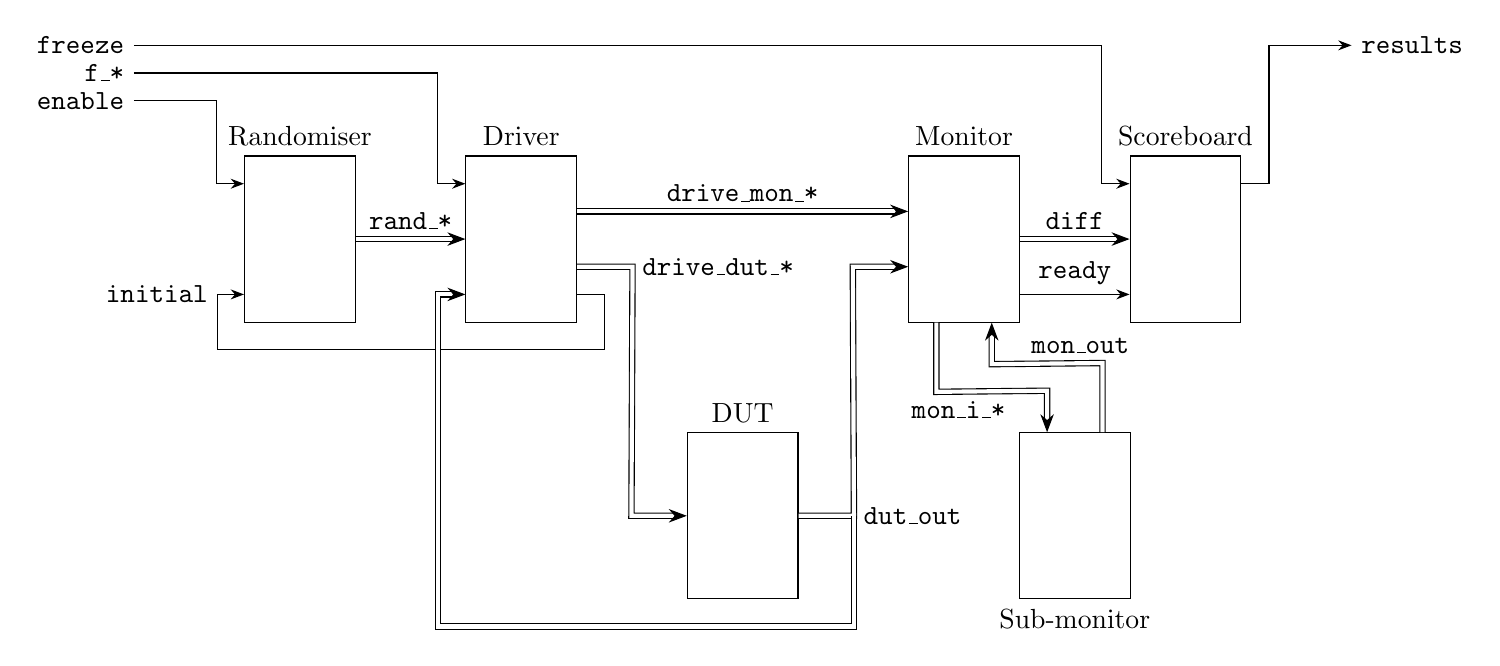
\begin{tikzpicture}
  [
    x=1em, y=1em,
    block/.style =
      {draw, rectangle, align=center, minimum width=4em, minimum height=6em},
    sarrow/.style =
      {>={Stealth}, font=\ttfamily},
    darrow/.style =
      {double distance=1.5pt, >={Stealth}, font=\ttfamily}
  ]
  \node [block, label=above:Randomiser]  at ( 8, 10)  (r) {};
  \node [block, label=above:Driver]      at (16, 10)  (d) {};
  \node [block, label=above:DUT]         at (24,  0)  (t) {};
  \node [block, label=above:Monitor]     at (32, 10)  (m) {};
  \node [block, label=below:Sub-monitor] at (36,  0)  (u) {};
  \node [block, label=above:Scoreboard]  at (40, 10)  (s) {};

  \draw [->, sarrow] (2,15) node[left] {enable}
                      -| ($(r.west)+(-1,2)$)
                      -- ($(r.west)+(0,2)$);
  \draw [->, sarrow] (2,16) node[left] {f\_*}
                      -| ($(d.west)+(-1,2)$)
                      -- ($(d.west)+(0,2)$);
  \draw [->, sarrow] (2,17) node[left] {freeze}
                      -| ($(s.west)+(-1,2)$)
                      -- ($(s.west)+(0,2)$);

  \draw [->, sarrow] ($(d.east)-(0,2)$)
                      -| ++(1,-2)
                      -- ++(-14,0)
                      |- node[left] {initial} ($(r.west)-(0,2)$);
  \draw [->, darrow] ($(r.east)+(0,0)$)
                      -- node[above] {rand\_*} ($(d.west)+(0,0)$);
  \draw [->, darrow] ($(d.east)+(0,1)$)
                      -- node[above] {drive\_mon\_*} ($(m.west)+(0,1)$);
  \draw [->, darrow] ($(d.east)-(0,1)$)
                      -- ++(2,0)
                      -- node[right,pos=0] {drive\_dut\_*} ($(t.west)+(-2,0)$)
                      -- ($(t.west)+(0,0)$);
  \draw [->, darrow] ($(t.east)-(0,0)$)
                      -- ++(2,0)
                      -- node[right,pos=0] {dut\_out} ($(m.west)-(2,1)$)
                      -- ($(m.west)-(0,1)$);
  \draw [->, darrow] ($(t.east)+(2,0)$)
                      |- ($(d.west)-(1,14)$)
                      |- ($(d.west)-(0,2)$);
  \draw [->, darrow] ($(m.south)-(1,0)$)
                      -- ++(0,-2.5)
                      -- node[below,pos=0.2] {mon\_i\_*} ($(u.north)-(1,-1.5)$)
                      -- ($(u.north)-(1,0)$);
  \draw [<-, darrow] ($(m.south)+(1,0)$)
                      -- ++(0,-1.5)
                      -- node[above,pos=0.8] {mon\_out} ($(u.north)+(1,2.5)$)
                      -- ($(u.north)+(1,0)$);
  \draw [->, darrow] ($(m.east)+(0,0)$)
                      -- node[above] {diff} ($(s.west)+(0,0)$);
  \draw [->, sarrow] ($(m.east)-(0,2)$)
                      -- node[above] {ready} ($(s.west)-(0,2)$);
  \draw [->, sarrow] ($(s.east)+(0,2)$)
                      -| ++(1,5)
                      -- (46,17) node[right] {results};

\end{tikzpicture}
    }
  \end{figure}
\end{frame}

\begin{frame}{Monitor Structure}
  \begin{itemize}
    \item Lazy Monitor
    \begin{itemize}
      \item Randomly selects data points to check
    \end{itemize}
  \end{itemize}
  \begin{figure}[H]
    \centering
    \resizebox{0.8\textwidth}{!}{%
      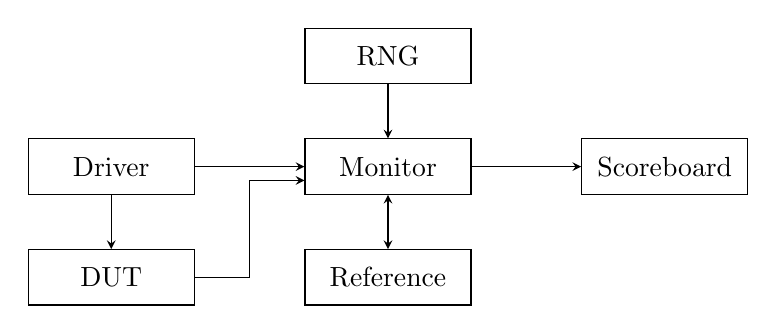
\begin{tikzpicture}
  [
    x=1em, y=1em,
    block/.style =
      {draw, rectangle, align=center, minimum width=6em, minimum height=2em},
    inter/.style =
      {draw, rectangle, align=center, minimum width=16em, minimum height=1em}
  ]
  \node [block] at ( 0,4)  (d) {Driver};
  \node [block] at ( 0,0)  (t) {DUT};
  \node [block] at (10,8)  (r) {RNG};
  \node [block] at (10,4)  (m) {Monitor};
  \node [block] at (10,0)  (u) {Reference};
  \node [block] at (20,4)  (s) {Scoreboard};

  \draw[ ->, >=stealth] (d.east)           -- (m.west);
  \draw[ ->, >=stealth] (d.south)          -- (t.north);
  \draw[ ->, >=stealth] (t.east)      to[-|-] ($(m.west)-(0,0.5)$);
  \draw[ ->, >=stealth] (r.south)          -- (m.north);
  \draw[<->, >=stealth] (m.south)          -- (u.north);
  \draw[ ->, >=stealth] (m.east)           -- (s.west);

\end{tikzpicture}
    }
  \end{figure}
\end{frame}

\begin{frame}[fragile]
  \frametitle{Software Design}
  \begin{columns}
  \column[t]{0.4\textwidth}
  \verbatimfont{\footnotesize}%
  \begin{verbatim}
mode: auto
bitset:
  a: 00000001
  b: 00000000
bitclr:
  a: 00000000
  b: 00000001
input:
  - a: 00000000
    b: 00000000
freq: 200
runtime: 60
  \end{verbatim}
  \column[t]{0.4\textwidth}
  \verbatimfont{\footnotesize}%
  \begin{verbatim}
> mode auto
> bitset a 00000001
> bitclr b 00000001
> freq 200
PLL Configured to 200.00MHz
> run 60
Results: ...
  \end{verbatim}
  \end{columns}
\end{frame}

\begin{frame}{REPL Commands}
  \begin{table}[H]
    \centering
    \begin{tabular}{|>{\ttfamily\scriptsize}p{8em}|>{\scriptsize}p{\dimexpr\textwidth-12em}|}
      \hline
      \textrm{Command}   & Explanation \\
      \hline
      reset              & Resets the system and test results. \\
      version            & Prints the system version. \\
      freq <speed>       & Sets the clock speed to the specified value in MHz. Prints the actual frequency configured. \\
      mode <m|a>         & Choose between \underline{m}anual and \underline{a}uto test mode. \\
      manual <a|b> <hex> & Give input in manual mode. \\
      bitset <a|b> <hex> & Force bits to be 1 in auto mode. \\
      bitclr <a|b> <hex> & Force bits to be 0 in auto mode. \\
      run <time>         & Runs the test for the duration specified in seconds. Prints the results at the end of the test. \\
      exit               & Exits the REPL. \\
      \hline
    \end{tabular}
  \end{table}
\end{frame}

\begin{frame}{Driver}
  \centering
  \resizebox{\textwidth}{!}{%
    \begin{tikztimingtable}
  [
    xscale=4,
    timing/d/background/.style={fill=white},
    timing/font=\ttfamily
  ]
  clk        & h 21{c} \\
  rand       & D{a4fe}D{527f}D{a93f}D{d49f}D{ea4f}D{7527}D{ba93}D{5d49}D{2ea4}D{1752}D{8ba9} \\
  f\_bitset  & 4D{0000} 7D{0004} \\
  f\_bitclr  & 3D{0000} 3D{f000} 5D{0000} \\
  drive\_dut & U D{a4fe}D{527f}D{a93f}D{049f}D{0a4f}D{0527}D{ba97}D{5d4d}D{1756}D{8bad} \\
  drive\_mon & 3U D{a4fe}D{527f}D{a93f}D{049f}D{0a4f}D{0527}D{ba97}D{5d4d} \\
  dut\_out   & 3U D{a4fe}D{527f}D{a93f}D{049f}D{0a4f}D{0527}D{ba97}D{5d4d} \\
\extracode
  % Add vertical lines in two colors
  \begin{pgfonlayer}{background}
    \begin{scope}[semitransparent,semithick]
      \vertlines{1,2,...,10}
    \end{scope}
  \end{pgfonlayer}
\end{tikztimingtable}
  }
\end{frame}

\begin{frame}{Monitor}
  \centering
  \resizebox{\textwidth}{!}{%
    \begin{tikztimingtable}
  [
    xscale=4,
    timing/d/background/.style={fill=white},
    timing/font=\ttfamily
  ]
  clk           & h 19{c} \\
  dist\_ctr     & D{100} 3{D{001}D{010}D{100}} \\
  drive\_mon\_a & U D{0123} 2U D{3210} 2U D{0213} 2U \\
  drive\_mon\_b & U D{4567} 2U D{7654} 2U D{4657} 2U \\
  dut\_out      & U D{468a} 2U D{a861} 2U D{486a} 2U \\
  clk\_sub  [0] & 2L 2{2{c} 2L} 2{c} L \\
  a         [0] & 2U 3D{0123} 3D{3210} 2D{0213} \\
  b         [0] & 2U 3D{4567} 3D{7654} 2D{4657} \\
  dut\_o    [0] & 2U 3D{468a} 3D{a861} 2D{486a} \\
  mon\_o    [0] & 2U 3D{468a} 3D{a864} 2D{486a} \\
  diff          & 2U 3U D{0000} 2U D{0005} U \\
\extracode
  % Add vertical lines in two colors
  \begin{pgfonlayer}{background}
    \begin{scope}[semitransparent,semithick]
      \vertlines{1,2,...,9}
    \end{scope}
  \end{pgfonlayer}
\end{tikztimingtable}
  }
\end{frame}

\begin{frame}{Scoreboard}
  \centering
  \resizebox{\textwidth}{!}{%
    \begin{tikztimingtable}
  [
    xscale=4,
    timing/d/background/.style={fill=white},
    timing/font=\ttfamily
  ]
  clk        & h 19{c} \\
  freeze     & 8L 2H \\
  mon\_ready & 2L 8H \\
  diff       & D{000f}D{0001}D{0000}D{0001}D{000c}2D{0000}3D{0001} \\
  data\_ctr  & 3D{0} 1R 6{Q} D{0} \\
  error\_ctr & 4D{0} D{1} 3D{2} D{3} D{4} \\
  maxacc     & 3D{0} 7D{16} \\
  minacc     & 3D{16} D{15} 6D{12} \\
\extracode
  % Add vertical lines in two colors
  \begin{pgfonlayer}{background}
    \begin{scope}[semitransparent,semithick]
      \vertlines{1,2,...,9}
    \end{scope}
  \end{pgfonlayer}
\end{tikztimingtable}
  }
\end{frame}

\end{document}